% ----------------------------------------------------
\begin{frame}
  \titlepage
\end{frame}
% ----------------------------------------------------
\note{Última sesión magistral del curso. Conectar con todo lo visto anteriormente: hemos cubierto actores, guerras, terrorismo, normas y DDHH, comercio, finanzas, desarrollo. Hoy cerramos mirando hacia adelante: los problemas que dominarán la política mundial en las próximas décadas. Dos grandes bloques temáticos: medio ambiente (capítulo 13 de FLS) y desafíos al orden internacional (capítulo 14). Son temas que conectan con todo lo anterior: bienes públicos, acción colectiva, instituciones, poder, conflicto. El objetivo es que los estudiantes apliquen las herramientas analíticas del curso a problemas actuales y futuros.}

% ----------------------------------------------------
\begin{frame}
\frametitle{Hoy}
\centering
\vspace{1.5em}
\begin{itemize}
  \setlength{\itemsep}{10pt}
  \item Medio ambiente: bienes públicos y acción colectiva
  \item El cambio climático como problema global
  \item Desafíos al orden liberal: populismo, migración y Ucrania
  \item Potencias emergentes: China y la transición de poder
  \item Armas, ciberamenazas e inteligencia artificial
\end{itemize}
\end{frame}
% ----------------------------------------------------
\note{}

% ====================================================
\section{El medio ambiente como bien público}
% ====================================================

% ----------------------------------------------------
\begin{transitionframe}
El medio ambiente como bien público
\end{transitionframe}
% ----------------------------------------------------
\note{}

% ----------------------------------------------------
\begin{frame}
\frametitle{¿Qué tipo de bien es el medio ambiente?}
\centering

\footnotesize
\begin{tabular}{>{\bfseries}l p{3.5cm} p{3.5cm}}
 & \textbf{Excluible} & \textbf{No excluible} \\[6pt]
\hline
Rival & Bien privado \newline \scriptsize (comida, ropa) & \textcolor{accent2}{\textbf{Recurso común}} \newline \scriptsize (pesca, bosques) \\[10pt]
No rival & Bien club \newline \scriptsize (TV por cable) & \textcolor{accent}{\textbf{Bien público}} \newline \scriptsize (aire limpio, capa de ozono) \\[6pt]
\end{tabular}

\vspace{10pt}
\onslide<2->{\small El medio ambiente combina características de \textbf{recurso común} y \textbf{bien público}}

\end{frame}
% ----------------------------------------------------
\note{Antes de hablar de medio ambiente, necesitamos entender qué tipo de bien es. Dos dimensiones clave: rivalidad (¿el consumo de uno reduce lo disponible para otros?) y excluibilidad (¿se puede impedir el acceso?). Un bien público puro es no rival y no excluible: el aire limpio, la estabilidad climática. Nadie puede ser excluido de respirar aire limpio, y que yo respire no reduce tu capacidad de hacerlo. Un recurso común (common pool resource) es rival pero no excluible: los bancos de pesca en alta mar, los bosques. Si yo pesco un atún, tú ya no puedes pescarlo, pero no puedo impedirte que pesques. El medio ambiente tiene características de ambos: la atmósfera es un bien público (todos nos beneficiamos de la capa de ozono), pero los recursos naturales son recursos comunes (la sobrepesca agota los caladeros). El problema es el mismo en ambos casos: los incentivos individuales llevan a la sobreexplotación.}

% ----------------------------------------------------
\begin{frame}
\frametitle{La tragedia de los comunes}
\centering
\vspace{0.5em}

\resizebox{0.85\textwidth}{!}{%
\begin{tikzpicture}[>=stealth, thick]
  % Central resource
  \node[draw, fill=accent!20, rounded corners, minimum width=3cm, minimum height=1.5cm, align=center] (res) at (0,0) {\textbf{Recurso común}\\\small (océano, atmósfera)};

  % Actors
  \node[draw, circle, fill=accent2!15, minimum size=1.2cm, align=center, font=\small] (a1) at (-4, 2) {Estado\\A};
  \node[draw, circle, fill=accent2!15, minimum size=1.2cm, align=center, font=\small] (a2) at (0, 3) {Estado\\B};
  \node[draw, circle, fill=accent2!15, minimum size=1.2cm, align=center, font=\small] (a3) at (4, 2) {Estado\\C};
  \node[draw, circle, fill=accent2!15, minimum size=1.2cm, align=center, font=\small] (a4) at (-3, -2.5) {Empresa\\X};
  \node[draw, circle, fill=accent2!15, minimum size=1.2cm, align=center, font=\small] (a5) at (3, -2.5) {Empresa\\Y};

  % Arrows (extraction)
  \draw[->, accent2, thick] (res) -- (a1) node[midway, left, font=\scriptsize] {extraer};
  \draw[->, accent2, thick] (res) -- (a2) node[midway, right, font=\scriptsize] {extraer};
  \draw[->, accent2, thick] (res) -- (a3) node[midway, right, font=\scriptsize] {extraer};
  \draw[->, accent2, thick] (res) -- (a4) node[midway, left, font=\scriptsize] {contaminar};
  \draw[->, accent2, thick] (res) -- (a5) node[midway, right, font=\scriptsize] {contaminar};

  % Label
  \node[font=\small\itshape, text=asher] at (0, -4) {Cada actor se beneficia individualmente, pero el recurso se agota};
\end{tikzpicture}}

\end{frame}
% ----------------------------------------------------
\note{La tragedia de los comunes (Hardin, 1968): cuando un recurso es compartido y no excluible, cada actor tiene incentivos para sobreexplotarlo. Ejemplo clásico: un pasto comunal. Cada ganadero tiene incentivos para añadir una vaca más: el beneficio es para él, pero el coste (deterioro del pasto) se reparte entre todos. Si todos hacen lo mismo, el pasto se destruye. Aplicado al medio ambiente: cada país tiene incentivos para contaminar (el beneficio económico es nacional) pero el coste (cambio climático, agotamiento de recursos) es global. Es un dilema del prisionero a gran escala: la cooperación beneficiaría a todos, pero cada actor tiene incentivos para ``hacer trampa.'' La diferencia con el dilema del prisionero clásico: aquí hay muchos actores, lo que hace la cooperación aún más difícil. Mencionar que Elinor Ostrom (Nobel 2009) demostró que las comunidades locales sí pueden gestionar recursos comunes sin privatización ni Estado --- pero a escala global es mucho más difícil.}

% ----------------------------------------------------
\begin{frame}
\frametitle{¿Qué facilita la cooperación medioambiental?}
\centering

\begin{itemize}
  \item<1-> \textbf{Número de actores:} cuantos menos, más fácil coordinar
  \begin{itemize}
    \item 2 países vs.~193 en la ONU
  \end{itemize}
  \item<2-> \textbf{Complejidad del problema:} problemas simples → soluciones simples
  \begin{itemize}
    \item Capa de ozono vs.~cambio climático
  \end{itemize}
  \item<3-> \textbf{Interacción repetida:} la sombra del futuro incentiva la cooperación
  \item<4-> \textbf{Productos conjuntos:} si cooperar tiene beneficios adicionales
  \begin{itemize}
    \item Reducir emisiones → menos dependencia del petróleo
  \end{itemize}
  \item<5-> \textbf{Grupos privilegiados:} un actor grande puede asumir el coste
  \begin{itemize}
    \item EE.UU.~liderando la prohibición del CFC
  \end{itemize}
\end{itemize}

\end{frame}
% ----------------------------------------------------
\note{Cinco factores del libro (FLS, cap.~13) que determinan si la cooperación medioambiental es posible. (1) Número de actores: la lluvia ácida entre EE.UU. y Canadá se resolvió relativamente rápido porque solo había dos partes. El cambio climático involucra a 193+ países. (2) Complejidad: el agujero de ozono tenía una causa clara (CFCs) y un sustituto disponible. El cambio climático implica toda la economía global. (3) Interacción repetida: las cumbres anuales del clima (COP) crean un juego repetido que facilita la reciprocidad. (4) Productos conjuntos: si reducir emisiones también mejora la salud pública o crea empleos verdes, hay más incentivos. (5) Grupos privilegiados: cuando un actor grande (como la UE en política climática) está dispuesto a liderar, puede arrastrar a otros. Estos cinco factores explican por qué algunos problemas medioambientales se resuelven (ozono) y otros no (clima).}

% ----------------------------------------------------
\begin{frame}
\frametitle{Caso de éxito: el Protocolo de Montreal (1987)}
\centering

\begin{columns}[T]
\begin{column}{0.47\textwidth}
\textcolor{accent}{\textbf{¿Por qué funcionó?}}
\begin{itemize}
  \setlength{\itemsep}{6pt}
  \item Problema científicamente claro
  \item Pocos productores de CFC
  \item Sustitutos disponibles (DuPont)
  \item EE.UU.~como líder
  \item Fondo para países en desarrollo
\end{itemize}
\end{column}
\begin{column}{0.47\textwidth}
\textcolor{accent2}{\textbf{¿Por qué el clima es diferente?}}
\begin{itemize}
  \setlength{\itemsep}{6pt}
  \item Causas múltiples y difusas
  \item Toda la economía mundial implicada
  \item No hay sustituto fácil
  \item Sin liderazgo claro
  \item Tensión Norte-Sur profunda
\end{itemize}
\end{column}
\end{columns}

\end{frame}
% ----------------------------------------------------
\note{El Protocolo de Montreal es probablemente el tratado medioambiental más exitoso de la historia. En 1985 se descubrió el agujero en la capa de ozono sobre la Antártida. En 1987 se firmó el Protocolo. Los CFCs se han reducido en más del 99\%. La capa de ozono se está recuperando y se espera su restauración completa hacia 2066. ¿Por qué funcionó? La ciencia era clara y el consenso rápido. Solo había unas pocas empresas químicas que producían CFCs (DuPont era la mayor) y ya tenían sustitutos en desarrollo. EE.UU.~lideró porque su propia industria estaba lista para la transición. Se creó un fondo multilateral para ayudar a países en desarrollo a hacer la transición. Contraste con el clima: las emisiones de CO2 vienen de absolutamente todo (transporte, industria, agricultura, calefacción). No hay un ``sustituto'' simple para los combustibles fósiles. EE.UU.~no ha liderado consistentemente (retirada del Protocolo de Kioto, retirada del Acuerdo de París bajo Trump). La tensión Norte-Sur es mucho más profunda.}

% ----------------------------------------------------
\begin{frame}
\frametitle{La tensión Norte-Sur}
\centering
\vspace{0.5em}

% \resizebox{0.8\textwidth}{!}{%
% \begin{tikzpicture}[>=stealth, thick]
%   % Two nodes
%   \node[draw, fill=accent!20, rounded corners, minimum width=3.5cm, minimum height=2cm, align=center] (north) at (-3.5,0) {\textbf{Norte global}\\\small (países ricos)\\\scriptsize Responsables históricos\\\scriptsize de las emisiones};
%   \node[draw, fill=accent2!15, rounded corners, minimum width=3.5cm, minimum height=2cm, align=center] (south) at (3.5,0) {\textbf{Sur global}\\\small (países en desarrollo)\\\scriptsize Sufren más los efectos\\\scriptsize pero necesitan crecer};

%   % Tension arrows
%   \draw[<->, very thick, accent2] (north) -- (south) node[midway, above, font=\small\bfseries] {Tensión};
%   \node[font=\scriptsize\itshape, text=asher, align=center] at (0, -1.2) {``¿Por qué debemos limitar nuestro crecimiento\\por un problema que vosotros causasteis?''};

%   % Bottom label
%   \node[draw, fill=accent!10, rounded corners, font=\small, align=center] at (0, -2.8) {\textbf{Responsabilidades comunes pero diferenciadas}\\\scriptsize (principio del Acuerdo de París)};
% \end{tikzpicture}}

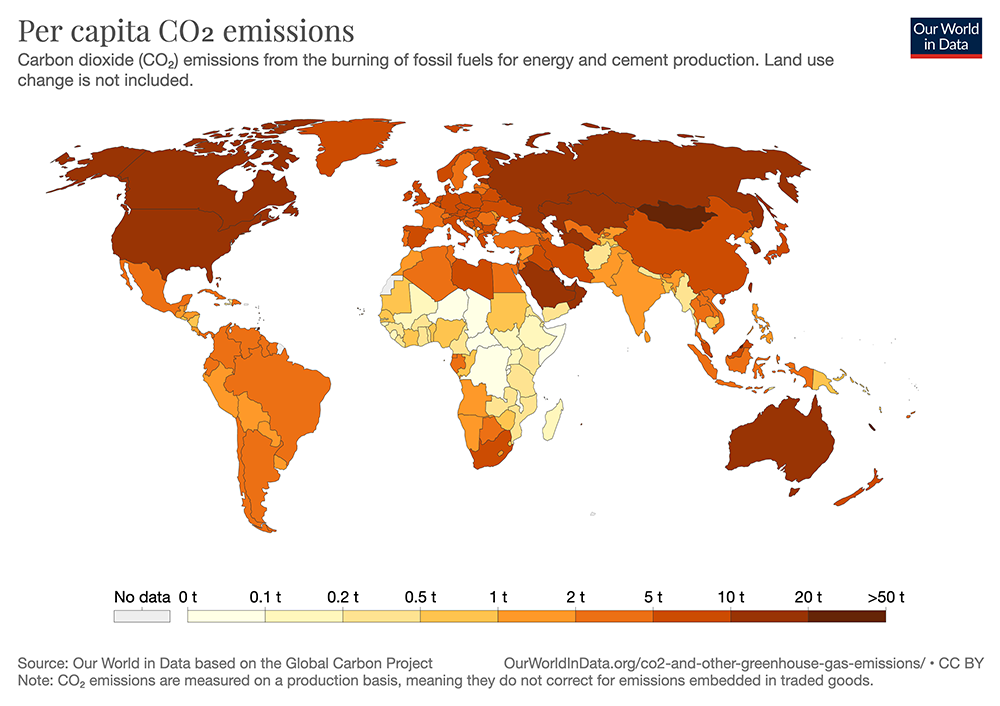
\includegraphics[width = \textwidth]{img/emissions_per_capita}


\end{frame}
% ----------------------------------------------------
\note{Una de las tensiones más profundas de la política medioambiental global. Los países ricos (EE.UU., UE, Japón) son responsables de la mayor parte de las emisiones históricas acumuladas. Los países en desarrollo (China, India, África) apenas están empezando a industrializarse y argumentan que tienen derecho al mismo desarrollo que tuvo Occidente. La India emite unas 2 toneladas de CO2 per cápita; EE.UU.~emite unas 15. ¿Es justo pedir a la India que limite su crecimiento? El principio de ``responsabilidades comunes pero diferenciadas'' intenta resolver esto: todos tienen que actuar, pero los ricos más y primero. En la práctica, esto se traduce en financiación climática: los países ricos prometen 100.000 millones de dólares anuales para ayudar a los países en desarrollo a hacer la transición energética. Hasta ahora, no se ha cumplido plenamente esa promesa. Esta tensión es un ejemplo perfecto de cómo los intereses divergentes dificultan la cooperación internacional incluso cuando todos reconocen el problema.}

% ----------------------------------------------------
\begin{frame}
\centering
\vspace{2em}
{\large ¿Por qué es tan difícil cooperar en medio ambiente si \textbf{todos} se beneficiarían de la cooperación?}
\vspace{1em}

\onslide<2->{\small Pensad en los cinco factores y en el dilema del prisionero}
\end{frame}
% ----------------------------------------------------
\note{Pregunta socrática para los estudiantes. Dejar 2-3 minutos para que piensen. Guiar la discusión hacia: (1) el problema del polizón (free-rider): cada país prefiere que los demás reduzcan emisiones mientras él sigue contaminando; (2) los costes son inmediatos pero los beneficios son a largo plazo y difusos; (3) la asimetría entre países: los que más contaminan (países ricos) no son los que más sufren (países pobres y estados insulares); (4) los grupos de interés domésticos: la industria del petróleo tiene más capacidad de organización que los ciudadanos preocupados por el clima; (5) la incertidumbre científica fue explotada durante décadas para justificar la inacción. Conectar con el concepto de externalidades: los costes de la contaminación los pagan terceros que no participan en la decisión de contaminar.}

% ====================================================
\section{El cambio climático}
% ====================================================

% ----------------------------------------------------
\begin{transitionframe}
El cambio climático
\end{transitionframe}
% ----------------------------------------------------
\note{}

% ----------------------------------------------------
\begin{frame}[plain]
  \begin{tikzpicture}[remember picture, overlay]
    \node[at = (current page.center), yshift = 0cm] (cover) {%
      \includegraphics[keepaspectratio, height=\paperheight]{../img/climate_warming_stripes}};
  \end{tikzpicture}
\end{frame}
% ----------------------------------------------------
% IMAGE NEEDED: climate_warming_stripes -- las "warming stripes" de Ed Hawkins (barras verticales de color azul a rojo mostrando el aumento de temperatura global desde 1850 hasta hoy); imagen icónica de la visualización del cambio climático
\note{Las ``warming stripes'' de Ed Hawkins (Universidad de Reading): cada barra representa un año, desde 1850 hasta hoy. El color va del azul (más frío que la media) al rojo (más caliente). La tendencia es inequívoca: el planeta se está calentando, y la aceleración desde los años 80 es dramática. La temperatura media global ha subido aproximadamente 1.1°C desde la era preindustrial. El Acuerdo de París fija como objetivo limitar el calentamiento a 1.5°C (idealmente) o 2°C (máximo). Con las políticas actuales, vamos camino de 2.5-3°C para finales de siglo. Cada décima de grado importa: la diferencia entre 1.5°C y 2°C implica cientos de millones de personas más expuestas a olas de calor extremas, la desaparición de los arrecifes de coral, y el aumento del nivel del mar.}

% ----------------------------------------------------
\begin{frame}
\frametitle{El cambio climático: ¿por qué es el caso más difícil?}
\centering

\begin{itemize}
  \item<1-> \textbf{Muchos actores:} 193+ Estados, miles de empresas
  \item<2-> \textbf{Problema complejo:} toda la economía mundial depende de combustibles fósiles
  \item<3-> \textbf{Costes inmediatos, beneficios lejanos:} reducir emisiones cuesta hoy, el beneficio es para las generaciones futuras
  \item<4-> \textbf{Asimetría:} los que más contaminan no son los que más sufren
  \item<5-> \textbf{Sin liderazgo estable:} EE.UU.~entra y sale de acuerdos
\end{itemize}

\vspace{8pt}
\onslide<5->{\small \textit{Es un dilema del prisionero con 193 jugadores, consecuencias a 50 años y costes asimétricos}}

\end{frame}
% ----------------------------------------------------
\note{Repasar por qué el cambio climático es el problema de acción colectiva más difícil de todos los vistos en el curso. Conectar con los cinco factores del slide anterior aplicándolos uno a uno. (1) Muchos actores: la negociación climática involucra a todos los países del mundo, cada uno con intereses diferentes. Arabia Saudí no quiere dejar de vender petróleo; las islas del Pacífico se hunden literalmente. (2) Complejidad: a diferencia del ozono, las emisiones de CO2 vienen de absolutamente todo --- transporte, industria, agricultura, calefacción, deforestación. No hay un ``interruptor'' que apagar. (3) Horizonte temporal: los políticos piensan en ciclos electorales de 4 años; el clima cambia en décadas. (4) Asimetría: Bangladesh contribuye el 0.4\% de las emisiones globales pero puede perder el 17\% de su territorio por la subida del nivel del mar. (5) Liderazgo: EE.UU. se retiró de Kioto (Bush, 2001) y de París (Trump, 2017 y 2025). China lidera en renovables pero sigue siendo el mayor emisor absoluto.}

% ----------------------------------------------------
\begin{frame}
\frametitle{Herramientas de política climática}
\centering

\footnotesize
\begin{tabularx}{\textwidth}{>{\bfseries}l L L}
 & \textbf{Ventajas} & \textbf{Inconvenientes} \\[4pt]
\hline
\textcolor{accent}{Impuesto al carbono} & Eficiente: pone precio a la contaminación & Políticamente impopular; difícil de armonizar globalmente \\[8pt]
\textcolor{accent}{Cap-and-trade} & Garantiza un límite de emisiones; flexible & Volatilidad de precios; lobbying por permisos gratuitos \\[8pt]
\textcolor{accent}{Regulación directa} & Clara y ejecutable & Costosa; no incentiva la innovación \\[8pt]
\textcolor{accent}{Subsidios verdes} & Popular; estimula innovación & Costoso para el Estado; puede subsidiar a ricos \\[4pt]
\end{tabularx}

\vspace{8pt}
\onslide<2->{\small En la práctica, la mayoría de países usa una \textbf{combinación} de herramientas}

\end{frame}
% ----------------------------------------------------
\note{Las cuatro grandes herramientas de política climática. (1) Impuesto al carbono: la solución preferida por los economistas. Pones un precio a cada tonelada de CO2 emitida y dejas que el mercado se ajuste. El problema: es políticamente tóxico. Los ``chalecos amarillos'' en Francia (2018) empezaron como protesta contra un aumento del impuesto al diésel. (2) Cap-and-trade (mercado de emisiones): el gobierno fija un techo total de emisiones y reparte permisos que las empresas pueden comprar y vender. La UE tiene el mayor mercado de carbono del mundo (EU ETS), funcionando desde 2005. China lanzó el suyo en 2021. (3) Regulación directa: prohibir ciertos combustibles, exigir estándares de eficiencia. La UE prohibirá la venta de coches de combustión nuevos en 2035. (4) Subsidios: la Inflation Reduction Act de Biden (2022) destinó 369.000 millones de dólares a energía limpia. Popular pero caro. En la práctica, todos los países usan una mezcla. La clave: cualquier herramienta es mejor que no hacer nada, pero ninguna es perfecta.}

% ----------------------------------------------------
\begin{frame}
\frametitle{El Acuerdo de París (2015)}
\centering

\begin{itemize}
  \item<1-> Objetivo: limitar el calentamiento a \textbf{1.5--2°C} sobre niveles preindustriales
  \item<2-> Mecanismo: contribuciones nacionales voluntarias (\textit{NDCs})
  \begin{itemize}
    \item Cada país decide su propio objetivo
    \item Revisión cada 5 años (``ratchet mechanism'')
  \end{itemize}
  \item<3-> \textcolor{accent}{Logro:} casi universal (195 partes, incluida China)
  \item<4-> \textcolor{accent2}{Límite:} sin mecanismo de cumplimiento vinculante
  \begin{itemize}
    \item Las promesas actuales llevan a $\sim$2.5--3°C
  \end{itemize}
\end{itemize}

\vspace{6pt}
\onslide<4->{\small \textit{¿Puede funcionar un acuerdo sin castigos por incumplimiento?}}

\end{frame}
% ----------------------------------------------------
\note{El Acuerdo de París (diciembre 2015) es el marco actual de la política climática global. A diferencia de Kioto (1997), que imponía objetivos obligatorios solo a los países ricos, París adopta un enfoque bottom-up: cada país presenta sus propias ``contribuciones determinadas a nivel nacional'' (NDCs). La genialidad de París: al ser voluntario, logró que casi todos se unieran (195 partes). La debilidad: al ser voluntario, nadie está obligado a cumplir. El ``mecanismo de trinquete'' (ratchet) obliga a revisar y aumentar las ambiciones cada 5 años, pero no hay sanciones si un país no cumple. El problema actual: sumando todas las NDCs, el mundo va camino de 2.5-3°C, muy por encima del objetivo. La pregunta socrática del final conecta con lo visto en la sesión de derecho internacional: ¿puede el derecho blando ser efectivo? La respuesta depende de la presión social, los mercados financieros (desinversión en fósiles) y la tecnología (si las renovables se abaratan lo suficiente, la transición se vuelve rentable sin necesidad de castigos).}

% ----------------------------------------------------
\begin{frame}
\frametitle{Política doméstica y medio ambiente}
\centering

\begin{columns}[T]
\begin{column}{0.47\textwidth}
\textcolor{accent2}{\textbf{Contaminadores}}
\begin{itemize}
  \setlength{\itemsep}{6pt}
  \item Pocos y organizados
  \item Pérdidas concentradas
  \item Lobby poderoso
  \item Amenaza de deslocalización
\end{itemize}
\end{column}
\begin{column}{0.47\textwidth}
\textcolor{accent}{\textbf{Público general}}
\begin{itemize}
  \setlength{\itemsep}{6pt}
  \item Muchos y dispersos
  \item Beneficios difusos
  \item Problema de acción colectiva
  \item Horizonte temporal largo
\end{itemize}
\end{column}
\end{columns}

\vspace{10pt}
\onslide<2->{\centering\small La \textbf{lógica de la acción colectiva} (Olson) explica\\por qué las políticas climáticas avanzan tan lento}

\end{frame}
% ----------------------------------------------------
\note{La política climática no se decide solo en cumbres internacionales: se decide en la política doméstica de cada país. Y aquí opera la lógica de la acción colectiva de Olson (1965): los grupos pequeños con intereses concentrados se organizan mejor que los grupos grandes con intereses difusos. La industria del petróleo, el carbón y el gas natural tiene mucho que perder con la regulación climática: son pocas empresas con mucho en juego, bien financiadas y con acceso directo a los gobiernos. ExxonMobil gastó décadas financiando estudios que cuestionaban la ciencia del clima. El público general se beneficiaría de un aire más limpio y un clima estable, pero cada ciudadano individual tiene poco incentivo para organizarse: el beneficio es difuso y lejano. Esto explica por qué las políticas climáticas avanzan tan lentamente incluso en democracias donde la mayoría de los ciudadanos dice apoyar la acción climática. Conectar con el concepto de externalidades: los contaminadores imponen costes a terceros (el resto del mundo, las generaciones futuras) que no participan en la decisión.}

% ====================================================
\section{Desafíos al orden liberal}
% ====================================================

% ----------------------------------------------------
\begin{transitionframe}
Desafíos al orden liberal
\end{transitionframe}
% ----------------------------------------------------
\note{}

% ----------------------------------------------------
\begin{frame}
\frametitle{El orden internacional de posguerra}
\centering

\begin{itemize}
  \item<1-> Construido desde 1945 bajo \textbf{liderazgo estadounidense}
  \item<2-> Cinco pilares:
  \begin{enumerate}
    \setlength{\itemsep}{4pt}
    \item \textbf{Soberanía} e integridad territorial
    \item \textbf{Seguridad colectiva} (ONU, OTAN)
    \item \textbf{Bretton Woods:} cooperación económica (FMI, BM, GATT/OMC)
    \item \textbf{Democracia} y derechos humanos como valores universales
    \item EE.UU.~como \textbf{hegemon} estabilizador
  \end{enumerate}
  \item<3-> Éxito relativo: sin guerra entre grandes potencias en 80 años
\end{itemize}

\end{frame}
% ----------------------------------------------------
\note{El orden liberal internacional (Liberal International Order, LIO) es el marco institucional construido tras la Segunda Guerra Mundial. Lo hemos visto a lo largo de todo el curso: la ONU (sesión sobre actores), las Convenciones de Ginebra y los DDHH (sesión sobre normas), el GATT/OMC y Bretton Woods (sesiones de comercio y finanzas). Los cinco pilares se refuerzan mutuamente: la seguridad colectiva reduce la incertidumbre, lo que facilita la cooperación económica, que a su vez hace la guerra más costosa. EE.UU.~como hegemon proporcionó bienes públicos: seguridad (paraguas nuclear, OTAN), mercados abiertos, dólar como moneda de reserva. El gran éxito: no ha habido guerra entre grandes potencias desde 1945, algo sin precedentes en la historia moderna. Pero este orden nunca fue perfecto (guerras proxy, dictaduras aliadas, desigualdad global) y hoy enfrenta desafíos desde múltiples frentes.}

% ----------------------------------------------------
\begin{frame}
\frametitle{Tres tipos de desafíos}
\centering
\vspace{0.5em}

\begin{enumerate}
  \item<1-> \textcolor{accent2}{\textbf{``Estados canallas'' y actores no estatales}}
  \begin{itemize}
    \item Corea del Norte, ISIS, terrorismo transnacional
  \end{itemize}
  \item<2-> \textcolor{accent}{\textbf{Potencias emergentes}}
  \begin{itemize}
    \item China, India, Rusia: ¿revisionistas o integrables?
  \end{itemize}
  \item<3-> \textcolor{accent2}{\textbf{Los ``perdedores'' de la globalización}}
  \begin{itemize}
    \item Trabajadores desplazados, comunidades desindustrializadas
    \item Reacción populista y nacionalista
  \end{itemize}
\end{enumerate}

\vspace{8pt}
\onslide<3->{\small \textcolor{asher}{\scriptsize (Frieden, Lake \& Schultz, cap.~14)}}

\end{frame}
% ----------------------------------------------------
\note{FLS identifica tres grupos que desafían el orden de posguerra. (1) Estados que rechazan las reglas: Corea del Norte (proliferación nuclear), Irán (antes del acuerdo de 2015), ISIS (actor no estatal que rechazaba todo el sistema de Estados). Estos son desafíos serios pero manejables: son actores relativamente pequeños. (2) Potencias emergentes, sobre todo China: no rechazan necesariamente el sistema, pero quieren más voz y voto. China se ha beneficiado enormemente del orden liberal (su crecimiento económico depende del comercio global) pero no comparte los valores democráticos ni quiere que EE.UU.~domine. La gran pregunta: ¿se puede integrar a China en el orden existente o hay que reconstruirlo? (3) Los perdedores de la globalización dentro de los propios países ricos: trabajadores industriales que perdieron sus empleos, comunidades rurales que se sienten abandonadas. Este tercer desafío es quizás el más peligroso porque viene de dentro: el Brexit, Trump, Le Pen, Vox, son expresiones de esta reacción.}

% ----------------------------------------------------
\begin{frame}[plain]
  \begin{tikzpicture}[remember picture, overlay]
    \node[at = (current page.center), yshift = 0cm] (cover) {%
      \includegraphics[keepaspectratio, height=\paperheight]{../img/globalization_winners_losers}};
  \end{tikzpicture}
\end{frame}
% ----------------------------------------------------
% IMAGE NEEDED: globalization_winners_losers -- el gráfico del "elefante" de Branko Milanovic, mostrando el crecimiento del ingreso real entre 1988-2008 por percentil de la distribución global de ingreso. El gráfico tiene forma de elefante: fuerte crecimiento en los percentiles medios (clases medias asiáticas), estancamiento en los percentiles 75-90 (clases medias occidentales), y fuerte crecimiento en el top 1%
\note{El ``gráfico del elefante'' de Branko Milanovic (2012) es una de las visualizaciones más influyentes de la economía política reciente. Muestra quién ha ganado y quién ha perdido con la globalización entre 1988 y 2008. Los grandes ganadores: las clases medias de Asia (China, India, Indonesia) --- los percentiles 40-60 de la distribución global --- que han visto su ingreso real crecer un 60-80\%. Los grandes perdedores: las clases medias-bajas de los países ricos (los percentiles 75-90 de la distribución global) --- trabajadores industriales de EE.UU., Reino Unido, Francia --- cuyo ingreso real apenas ha crecido. Y el top 1\% global también ha ganado enormemente. La forma del gráfico se parece a un elefante: la trompa levantada a la derecha es el 1\% más rico. Este gráfico ayuda a entender el Brexit, Trump, el auge de la extrema derecha en Europa: no es irracionalidad, es una respuesta a décadas de estancamiento económico en sectores que antes eran prósperos.}

% ----------------------------------------------------
\begin{frame}
\frametitle{La reacción populista}
\centering

\begin{columns}[T]
\begin{column}{0.47\textwidth}
\textcolor{accent2}{\textbf{Populismo de derecha}}
\begin{itemize}
  \setlength{\itemsep}{6pt}
  \item Anti-inmigración
  \item Nacionalismo cultural
  \item Proteccionismo económico
  \item Desconfianza en OOII
  \item Trump, Brexit, Le Pen
\end{itemize}
\end{column}
\begin{column}{0.47\textwidth}
\textcolor{accent}{\textbf{Populismo de izquierda}}
\begin{itemize}
  \setlength{\itemsep}{6pt}
  \item Anti-élites económicas
  \item Redistribución radical
  \item Crítica a la austeridad
  \item Ambivalencia con OOII
  \item Podemos, Syriza, Sanders
\end{itemize}
\end{column}
\end{columns}

\vspace{10pt}
\onslide<2->{\centering\small Ambos comparten: desconfianza en las \textbf{élites} y las \textbf{instituciones establecidas}}

\end{frame}
% ----------------------------------------------------
\note{El populismo no es un fenómeno uniforme. La distinción izquierda-derecha importa mucho en la práctica, aunque ambos comparten una estructura retórica: ``el pueblo'' virtuoso contra ``las élites'' corruptas. El populismo de derecha tiende a definir ``el pueblo'' en términos culturales o étnicos (los ``verdaderos'' americanos, franceses, etc.) y percibe la amenaza en los inmigrantes y las instituciones supranacionales. El populismo de izquierda define ``el pueblo'' en términos económicos (los trabajadores, el 99\%) y percibe la amenaza en las élites financieras y las corporaciones multinacionales. Ambos desconfían de las instituciones internacionales (OMC, UE, FMI), pero por razones diferentes: la derecha las ve como amenaza a la soberanía nacional; la izquierda las ve como instrumentos del capital global. Para la política mundial, el populismo de derecha es más directamente desestabilizador porque cuestiona los pilares del orden liberal: libre comercio, multilateralismo, alianzas militares. Trump retiró a EE.UU.~del Acuerdo de París, impuso aranceles, cuestionó la OTAN.}

% ----------------------------------------------------
\begin{frame}
\centering
\vspace{2em}
{\large ¿Es el populismo una \textbf{amenaza} para la democracia\\ o una \textbf{respuesta legítima} a la desigualdad?}
\end{frame}
% ----------------------------------------------------
\note{Segunda pregunta socrática. Dejar 2-3 minutos para que piensen. Argumentos a favor de que es una amenaza: erosión de normas democráticas (ataques a la prensa, al poder judicial, a las minorías), polarización extrema, rechazo del compromiso democrático. Ejemplos: Hungría bajo Orbán, Venezuela bajo Chávez/Maduro, el asalto al Capitolio en enero de 2021. Argumentos a favor de que es una respuesta legítima: las democracias liberales no han respondido adecuadamente a la desigualdad creciente, a la desindustrialización, a la inseguridad económica. Si las instituciones democráticas no canalizan el descontento, este busca otros cauces. La respuesta más matizada: el populismo como síntoma es legítimo (señala problemas reales); el populismo como solución es peligroso (tiende a erosionar los contrapesos institucionales). Conectar con Dani Rodrik y su ``trilema de la globalización'': no puedes tener simultáneamente globalización económica, soberanía nacional y democracia. El populismo surge cuando la globalización avanza y la democracia no compensa a los perdedores.}

% ----------------------------------------------------
\begin{frame}
\frametitle{Migración: el desafío ausente}
\centering

\begin{itemize}
  \item $\sim$\textbf{280 millones} de migrantes internacionales (2023) --- el 3,6\% de la población mundial
  \vspace{6pt}
  \item<2-> La economía es clara: la migración genera \textbf{ganancias netas}
  \begin{itemize}
    \item Trabajadores llenan vacantes, pagan impuestos, innovan
    \item Remesas: $\sim$650.000 M\$/año --- más que toda la ayuda al desarrollo
  \end{itemize}
  \vspace{6pt}
  \item<3-> Pero la política es explosiva:
  \begin{itemize}
    \item \textbf{Distribución desigual} de costes y beneficios (como el comercio)
    \item Dimensión \textbf{cultural e identitaria}: no solo económica
    \item Principal bandera del \textbf{populismo de derecha} en Europa y EE.UU.
  \end{itemize}
  \vspace{6pt}
  \item<4-> \alert{Paradoja:} no hay gobernanza global de la migración comparable al comercio (OMC) o las finanzas (FMI)
\end{itemize}

\end{frame}
% ----------------------------------------------------
\note{La migración es quizás el tema más políticamente explosivo de la política mundial contemporánea, y sin embargo carece de las instituciones internacionales que gobiernan otros flujos transfronterizos. Los bienes tienen la OMC, el capital tiene el FMI, pero las personas no tienen un equivalente. Los datos: 280 millones de migrantes internacionales, un número que crece pero sigue siendo un porcentaje modesto de la población mundial. Las remesas que envían (650.000 millones de dólares al año) superan con creces toda la ayuda al desarrollo, lo que las convierte en el mayor mecanismo de transferencia de renta del mundo. La economía de la migración es parecida a la del comercio: genera ganancias netas pero también ganadores y perdedores. Los empleadores y los consumidores se benefician; los trabajadores nativos que compiten directamente con los inmigrantes pueden verse perjudicados (aunque la evidencia empírica sobre esto es más débil de lo que se cree). Pero la migración tiene una dimensión que el comercio no tiene: la identidad cultural. El debate sobre inmigración no es solo sobre salarios y empleo; es sobre quién pertenece a la comunidad política. Esta dimensión cultural explica por qué la inmigración es la bandera número uno del populismo de derecha en todo el mundo desarrollado.}

% ----------------------------------------------------
\begin{frame}
\frametitle{Ucrania: el retorno de la guerra interestatal}
\centering

\begin{itemize}
  \item \textbf{Febrero 2022:} Rusia invade Ucrania --- la mayor guerra en Europa desde 1945
  \vspace{6pt}
  \item<2-> Desafío directo al orden de posguerra:
  \begin{itemize}
    \item Violación de la \textbf{soberanía} e integridad territorial
    \item Amenazas \textbf{nucleares} explícitas de Rusia
    \item Fracaso de la disuasión y de la ONU
  \end{itemize}
  \vspace{6pt}
  \item<3-> Respuesta occidental: \textbf{sanciones} sin precedentes
  \begin{itemize}
    \item \textit{Interdependencia armada} en acción: SWIFT, reservas congeladas
    \item Pero Rusia tiene recursos energéticos y aliados (China, India)
  \end{itemize}
  \vspace{6pt}
  \item<4-> Lecciones:
  \begin{itemize}
    \item La guerra interestatal \alert{no es cosa del pasado}
    \item La interdependencia económica \textbf{no garantiza la paz}
    \item Las armas nucleares disuaden la intervención directa pero no la guerra convencional
  \end{itemize}
\end{itemize}

\end{frame}
% ----------------------------------------------------
\note{La invasión rusa de Ucrania en febrero de 2022 es probablemente el acontecimiento más significativo de la política mundial desde el 11-S. Desafía tres supuestos centrales del orden de posguerra. Primero, la soberanía: la invasión viola el principio más básico del sistema de Estados (sesión sobre normas). Segundo, la disuasión: ni las sanciones previas ni la presencia de la OTAN impidieron la invasión, aunque sí impidieron la intervención directa occidental (por el riesgo nuclear). Tercero, la interdependencia: Rusia y Europa estaban profundamente interconectadas por el gas y el petróleo. La teoría liberal predecía que esta interdependencia haría la guerra irracional. No fue así. Esto conecta directamente con Farrell y Newman: la interdependencia no solo puede fallar como mecanismo de paz, sino que puede ser instrumentalizada como arma. Las sanciones contra Rusia son el mayor caso de interdependencia armada de la historia. Pero también muestran los límites: Rusia redirigió exportaciones energéticas hacia China e India, y la guerra continúa. La lección más profunda: las armas nucleares crean una paradoja. Disuaden la guerra directa entre potencias nucleares, pero al hacerlo, crean un paraguas bajo el cual la guerra convencional es posible (Rusia invade sabiendo que la OTAN no intervendrá directamente por miedo a la escalada nuclear).}

% ====================================================
\section{Potencias emergentes y transición de poder}
% ====================================================

% ----------------------------------------------------
\begin{transitionframe}
Potencias emergentes y transición de poder
\end{transitionframe}
% ----------------------------------------------------
\note{}

% ----------------------------------------------------
\begin{frame}[plain]
  \begin{tikzpicture}[remember picture, overlay]
    \node[at = (current page.center), yshift = 0cm] (cover) {%
      \includegraphics[keepaspectratio, height=\paperheight]{../img/china_usa_flags}};
  \end{tikzpicture}
\end{frame}
% ----------------------------------------------------
% IMAGE NEEDED: china_usa_flags -- imagen de las banderas de China y Estados Unidos juntas, simbolizando la rivalidad geopolítica; puede ser una foto de una cumbre bilateral o las banderas una junto a la otra
\note{China y EE.UU.: la rivalidad que definirá el siglo XXI. Imagen de transición para introducir la sección sobre potencias emergentes y transición de poder. Mencionar que esta es probablemente la dinámica geopolítica más importante de nuestro tiempo: cómo gestionar la relación entre una potencia establecida (EE.UU.) y una potencia emergente (China) que aspira a un papel mayor en el sistema internacional. La historia ofrece precedentes preocupantes (Atenas vs.~Esparta, Alemania vs.~Reino Unido) pero también esperanzadores (EE.UU.~vs.~Reino Unido en el siglo XIX, donde la transición fue pacífica).}

% ----------------------------------------------------
\begin{frame}
\frametitle{El ascenso de China}
\centering
\vspace{0.3em}

\resizebox{\textwidth}{!}{%
\begin{tikzpicture}[>=stealth, thick]
  % Timeline
  \draw[very thick, ->] (0,0) -- (14,0);

  % Year ticks
  \foreach \x/\year in {0.5/1978, 3/1989, 5/2001, 7.5/2008, 9.5/2013, 12/2020} {
    \draw (\x, -0.15) -- (\x, 0.15);
    \node[below, font=\scriptsize] at (\x, -0.2) {\year};
  }

  % Events (alternating above/below)
  \node[above, align=center, font=\scriptsize, text width=2cm] at (0.5, 0.4) {Reformas\\de Deng\\Xiaoping};
  \node[above, align=center, font=\scriptsize, text width=2cm] at (3, 1.4) {Tiananmen\\represión};
  \node[above, align=center, font=\scriptsize, text width=2cm] at (5, 0.4) {Entrada\\en la OMC};
  \node[above, align=center, font=\scriptsize, text width=2.5cm] at (7.5, 1.4) {Crisis financiera\\global};
  \node[above, align=center, font=\scriptsize, text width=2.5cm] at (9.5, 0.4) {Xi Jinping\\Belt \& Road};
  \node[above, align=center, font=\scriptsize, text width=2.5cm] at (12, 1.4) {Rivalidad\\tecnológica\\con EE.UU.};

  % Growth band
  \fill[accent!20] (0.5, -0.8) rectangle (12, -1.3);
  \node[font=\scriptsize\itshape, text=accent!80!black] at (6.25, -1.05) {PIB × 40 en cuatro décadas (crecimiento medio $\sim$10\% anual)};
\end{tikzpicture}}

\end{frame}
% ----------------------------------------------------
\note{Timeline del ascenso de China como potencia global. 1978: Deng Xiaoping inicia las reformas económicas (``socialismo de mercado''). China pasa de una economía planificada y aislada a la fábrica del mundo. 1989: Tiananmen muestra que la apertura económica no conlleva apertura política. 2001: China entra en la OMC, integrándose plenamente en el comercio global. Entre 2001 y 2008, su PIB se triplica. 2008: la crisis financiera global debilita a Occidente y refuerza el modelo chino (el gobierno inyecta un estímulo masivo). 2013: Xi Jinping consolida el poder y lanza Belt and Road Initiative (nueva Ruta de la Seda), el mayor proyecto de infraestructura de la historia. 2020 en adelante: la rivalidad tecnológica con EE.UU.~se intensifica (guerra de chips, Huawei, TikTok, IA). En 2024, China es la segunda economía del mundo por PIB nominal y la primera por PIB en paridad de poder adquisitivo. Su gasto militar ha crecido exponencialmente. La pregunta: ¿puede el sistema internacional absorber este ascenso pacíficamente?}

% ----------------------------------------------------
\begin{frame}
\frametitle{La teoría de la transición de poder}
\centering

\begin{itemize}
  \item<1-> Cuando una potencia \textbf{emergente} se acerca al poder de la \textbf{potencia dominante}, el riesgo de guerra aumenta
  \item<2-> ¿Por qué?
  \begin{itemize}
    \item El hegemón puede preferir una \textbf{guerra preventiva} antes de perder su ventaja
    \item La potencia emergente puede exigir cambios que el hegemón no acepta
  \end{itemize}
  \item<3-> Precedentes históricos:
  \begin{itemize}
    \item Atenas vs.~Esparta → Guerra del Peloponeso
    \item Alemania vs.~Reino Unido → Primera Guerra Mundial
  \end{itemize}
  \item<4-> Graham Allison (2017): la ``\textbf{trampa de Tucídides}''
\end{itemize}

\end{frame}
% ----------------------------------------------------
\note{La teoría de la transición de poder (Organski, 1958; ampliada por Gilpin, 1981) es una de las teorías más influyentes (y preocupantes) de las RRII. La idea básica: el sistema internacional tiende a ser estable cuando hay una potencia claramente dominante (hegemon). Pero cuando otra potencia crece y se acerca al nivel de poder del hegemon, se abre una ventana de peligro. El hegemon puede calcular que es mejor luchar ahora (cuando todavía tiene ventaja) que esperar a que el rival lo supere. Y la potencia emergente puede calcular que las reglas del juego están sesgadas a favor del hegemon y exigir cambios. Graham Allison (Harvard) estudió 16 casos históricos de transición de poder: en 12 de ellos, el resultado fue la guerra. Lo llamó la ``trampa de Tucídides,'' en referencia al historiador griego que escribió sobre la guerra entre Atenas (potencia emergente) y Esparta (potencia establecida). El paralelo China-EE.UU.~es obvio e inquietante.}

% ----------------------------------------------------
\begin{frame}
\frametitle{¿Es la guerra inevitable?}
\centering

\begin{itemize}
  \item<1-> \textbf{No necesariamente.} Tres factores diferenciadores:
  \item<2-> \textcolor{accent}{\textbf{Armas nucleares:}} la destrucción mutua asegurada (MAD) hace la guerra directa irracional
  \item<3-> \textcolor{accent}{\textbf{Interdependencia económica:}} EE.UU.~y China son socios comerciales masivos
  \begin{itemize}
    \item El coste de una guerra sería astronómico para ambos
  \end{itemize}
  \item<4-> \textcolor{accent}{\textbf{Instituciones internacionales:}} canales de comunicación, reglas compartidas
  \begin{itemize}
    \item ONU, OMC, G20, acuerdos bilaterales
  \end{itemize}
\end{itemize}

\vspace{8pt}
\onslide<4->{\small \textit{El modelo de negociación sugiere que la guerra es evitable\\si ambos lados pueden negociar y hacer concesiones}}

\end{frame}
% ----------------------------------------------------
\note{Contraargumentos a la inevitabilidad de la guerra. El modelo de negociación (bargaining model of war, visto en la sesión 3) sugiere que la guerra ocurre cuando hay información incompleta, problemas de compromiso o indivisibilidad. En el caso EE.UU.-China: (1) Las armas nucleares cambian fundamentalmente el cálculo. Ninguna potencia nuclear ha ido a la guerra directa contra otra potencia nuclear. La MAD (destrucción mutua asegurada) funciona como disuasión. (2) La interdependencia económica: EE.UU.~y China comercian por valor de más de 700.000 millones de dólares al año. China posee más de un billón de dólares en deuda estadounidense. Una guerra destruiría las cadenas de suministro globales. (3) Las instituciones: a diferencia de 1914 (Alemania vs.~Reino Unido), hoy existe una densa red de instituciones que facilita la comunicación y reduce la incertidumbre. Los 4 casos de transición pacífica de Allison tienen algo en común: instituciones fuertes y capacidad de negociar. Mención a Taiwán como el punto más peligroso: es la cuestión donde los intereses son más difíciles de negociar.}

% ----------------------------------------------------
\begin{frame}
\centering
\vspace{2em}
{\large ¿Podrán EE.UU.~y China evitar la ``trampa de Tucídides''?\\[10pt] ¿Qué factores juegan a favor y en contra?}
\end{frame}
% ----------------------------------------------------
\note{Tercera pregunta socrática. Factores a favor de la paz: armas nucleares, interdependencia económica, instituciones, experiencia histórica (ambos conocen los riesgos). Factores en contra: Taiwán (potencial detonante), competencia tecnológica (IA, semiconductores), nacionalismo en ambos países, desconfianza mutua creciente, la lógica de la trampa de Tucídides. Preguntar a los estudiantes: ¿qué piensan que es más importante, los factores estructurales (poder relativo) o los factores institucionales (reglas, comunicación)? Conectar con el debate realismo vs.~liberalismo visto al principio del curso: los realistas dirán que la estructura de poder determina el conflicto; los liberales dirán que las instituciones y la interdependencia pueden prevenirlo.}

% ====================================================
\section{Armas, proliferación y ciberamenazas}
% ====================================================

% ----------------------------------------------------
\begin{transitionframe}
Armas, proliferación y ciberamenazas
\end{transitionframe}
% ----------------------------------------------------
\note{}

% ----------------------------------------------------
\begin{frame}
\frametitle{Disuasión nuclear: ¿cómo funciona?}
\centering

\begin{itemize}
  \item<1-> \textbf{Destrucción mutua asegurada} (MAD):
  \begin{itemize}
    \item Si A ataca a B, B puede responder con un \textbf{segundo golpe} devastador
    \item → Ningún actor racional inicia un ataque nuclear
  \end{itemize}
  \item<2-> Tres condiciones necesarias:
  \begin{enumerate}
    \setlength{\itemsep}{4pt}
    \item \textbf{Capacidad de segundo golpe:} sobrevivir al primer ataque (submarinos, silos)
    \item \textbf{Racionalidad:} ambos líderes son racionales
    \item \textbf{Verificabilidad:} cada lado sabe que el otro puede responder
  \end{enumerate}
  \item<3-> Resultado: \textbf{paz por terror} --- estabilidad paradójica
\end{itemize}

\end{frame}
% ----------------------------------------------------
\note{La disuasión nuclear es uno de los conceptos más contraintuitivos de las RRII: las armas más destructivas de la historia han producido la paz más larga entre grandes potencias. La lógica de la MAD (Mutual Assured Destruction): si ambos bandos pueden destruirse mutuamente incluso después de recibir un primer golpe, ninguno tiene incentivos para atacar primero. La capacidad de segundo golpe es crucial: por eso los submarinos nucleares son tan importantes (son casi imposibles de localizar y destruir simultáneamente). La racionalidad es un supuesto fuerte: ¿qué pasa si un líder no es racional o si hay un error técnico? El teléfono rojo Moscú-Washington se creó precisamente para reducir el riesgo de guerra accidental. La verificabilidad se logra mediante satélites espía y tratados de control de armas (START) que permiten inspecciones mutuas. La paradoja: las armas nucleares han sido probablemente el mayor factor de paz entre grandes potencias desde 1945. Kenneth Waltz argumentaba que ``más sería mejor'' (más países con armas nucleares = más estabilidad), pero la mayoría de expertos discrepa.}

% ----------------------------------------------------
\begin{frame}
\frametitle{¿Por qué nuevos Estados nucleares son diferentes?}

\small Tres razones por las que la proliferación preocupa:

\begin{itemize}
  \setlength{\itemsep}{8pt}
  \item<2-> \textbf{1. Instituciones débiles:} cadenas de mando frágiles, riesgo de uso no autorizado (ej.~Pakistán)
  \item<3-> \textbf{2. Sin segundo golpe seguro:} arsenales pequeños y vulnerables → incentivos para ``usar o perder''
  \item<4-> \textbf{3. Riesgo de transferencia:} tecnología puede llegar a actores no estatales (red de A.Q.~Khan: Pakistán → Libia, Irán, Corea del Norte)
\end{itemize}

\end{frame}
% ----------------------------------------------------
\note{El argumento de Waltz (``más sería mejor'') asume que todos los nuevos Estados nucleares se comportarán como EE.UU.~y la URSS: racionalmente, con instituciones sólidas y capacidad de segundo golpe segura. Pero hay tres razones para dudar. (1) Las instituciones de mando y control son mucho más débiles en países como Pakistán o Corea del Norte. En EE.UU., hay múltiples capas de autorización antes de poder lanzar un arma nuclear. En Pakistán, hay dudas sobre quién tendría realmente la autoridad en una crisis. Un golpe militar podría poner las armas en manos impredecibles. (2) Los arsenales pequeños son más vulnerables a un primer golpe, lo que crea una lógica de ``usar o perder'': si crees que tu enemigo puede destruir tus 10 misiles en un primer ataque, tienes incentivos para lanzarlos antes de perderlos. EE.UU.~y la URSS tenían miles de cabezas nucleares distribuidas en tierra, mar y aire; Corea del Norte tiene quizás 40-50. (3) La red de A.Q.~Khan demostró que un científico nuclear pakistaní podía vender tecnología y planos a Libia, Irán y Corea del Norte durante años sin que el gobierno pakistaní (supuestamente) lo supiera. Si la tecnología nuclear se difunde a actores no estatales, la disuasión no funciona: no puedes amenazar con represalia nuclear a un grupo terrorista sin Estado.}

% ----------------------------------------------------
\begin{frame}
\frametitle{El Tratado de No Proliferación (TNP)}
\centering

\begin{columns}[T]
\begin{column}{0.47\textwidth}
\textcolor{accent}{\textbf{Éxitos}}
\begin{itemize}
  \setlength{\itemsep}{6pt}
  \item 191 Estados parte
  \item En los 60 se temían 25+ Estados nucleares; hoy son 9
  \item Sudáfrica, Brasil, Argentina renunciaron
  \item Inspecciones del OIEA
\end{itemize}
\end{column}
\begin{column}{0.47\textwidth}
\textcolor{accent2}{\textbf{Fracasos}}
\begin{itemize}
  \setlength{\itemsep}{6pt}
  \item India, Pakistán, Israel nunca firmaron
  \item Corea del Norte se retiró (2003)
  \item Irán: programa clandestino
  \item Los 5 nucleares legítimos no desarman
\end{itemize}
\end{column}
\end{columns}

\vspace{8pt}
\onslide<2->{\centering\small El TNP es un \textbf{éxito relativo} notable pero con fallos espectaculares}

\end{frame}
% ----------------------------------------------------
\note{El Tratado de No Proliferación Nuclear (TNP, 1968) es uno de los regímenes internacionales más exitosos. En los años 60, Kennedy predijo que para los 70 habría 25 o más Estados nucleares. Hoy hay 9 (EE.UU., Rusia, Reino Unido, Francia, China --- los 5 ``legítimos'' del TNP --- más India, Pakistán, Israel y Corea del Norte). El TNP descansa en un gran acuerdo: los 5 nucleares prometen desarmar (artículo VI) y los demás prometen no adquirir armas nucleares, a cambio de acceso a tecnología nuclear civil. El OIEA (Organismo Internacional de Energía Atómica) verifica el cumplimiento mediante inspecciones. Los éxitos: Sudáfrica construyó 6 bombas nucleares durante el apartheid y luego las desmanteló voluntariamente (único caso). Brasil y Argentina abandonaron sus programas en los años 90. Libia renunció en 2003. Los fracasos: India (pruebas en 1974 y 1998), Pakistán (1998) e Israel (nunca confirmado pero universalmente aceptado) nunca firmaron. Corea del Norte firmó, se retiró en 2003 y realizó 6 pruebas nucleares. Irán desarrolló un programa clandestino que el acuerdo de 2015 (JCPOA) intentó frenar, pero Trump se retiró del acuerdo en 2018.}

% ----------------------------------------------------
\begin{frame}
\frametitle{Ciberamenazas: la nueva frontera}

\begin{itemize}
  \setlength{\itemsep}{8pt}
  \item<1-> \textbf{Características únicas} de las ciberarmas:
  \begin{itemize}
    \item Difícil \textbf{atribución}: ¿quién atacó?
    \item Actores no estatales con gran capacidad
    \item Bajo coste de entrada, alto impacto potencial
  \end{itemize}
  \item<2-> ¿Por qué la disuasión \textbf{no funciona} igual?
  \begin{itemize}
    \item No sabes quién te atacó → no puedes represaliar
    \item Zona gris: ¿es un acto de guerra o espionaje?
  \end{itemize}
\end{itemize}

\end{frame}
% ----------------------------------------------------
\note{Las ciberarmas representan un desafío fundamentalmente nuevo. A diferencia de las armas convencionales o nucleares, tienen características que complican la disuasión. (1) Atribución: cuando un misil cae, sabes de dónde viene. Un ciberataque puede tardar meses en atribuirse. Rusia niega su implicación en hackeos que múltiples agencias le atribuyen. (2) Actores no estatales: un grupo de hackers con pocos recursos puede causar daños enormes. WannaCry (2017) afectó a 200.000 ordenadores en 150 países. (3) Zona gris: ¿un ciberataque contra una central eléctrica es un acto de guerra? No hay normas claras.}

% ----------------------------------------------------
\begin{frame}
\frametitle{Ciberataques: ejemplos}

\begin{itemize}
  \setlength{\itemsep}{10pt}
  \item<1-> \textbf{Stuxnet} (2010): virus de EE.UU./Israel destruyó centrifugadoras nucleares iraníes --- sabotaje sin disparar un tiro
  \item<2-> \textbf{Hackeos rusos} en elecciones de EE.UU.~(2016): interferencia electoral como herramienta geopolítica
  \item<3-> \textbf{Ransomware}: ataques contra hospitales e infraestructuras críticas por lucro o desestabilización
\end{itemize}

\vspace{8pt}
\onslide<4->{\centering\small\textit{La lógica de la disuasión nuclear no se traslada al ciberespacio}}

\end{frame}
% ----------------------------------------------------
\note{Stuxnet es el caso más famoso: un virus informático (atribuido a EE.UU.~e Israel) destruyó centrifugadoras nucleares iraníes. Fue un acto de sabotaje que retrasó el programa nuclear iraní 2 años, pero se hizo sin disparar un solo tiro. ¿Tenía Irán derecho a represaliar militarmente? No hay consenso. Los hackeos rusos en las elecciones de 2016 mostraron que el ciberespacio puede usarse para interferir en la democracia de otros países. Y el ransomware (como WannaCry, atribuido a Corea del Norte) demostró que actores estatales y no estatales pueden paralizar hospitales y servicios públicos. La conclusión clave: la lógica de la disuasión que funciona con armas nucleares no se traslada al ciberespacio, porque falta la atribución clara y la capacidad de represalia creíble.}

% ----------------------------------------------------
\begin{frame}
\frametitle{Inteligencia artificial: la nueva carrera geopolítica}
\centering

\begin{itemize}
  \item<1-> La IA como \textbf{tecnología transformadora} --- comparable a la electricidad o la energía nuclear
  \vspace{6pt}
  \item<2-> \textbf{Dimensión militar:}
  \begin{itemize}
    \item Armas autónomas, drones con IA, ciberdefensa automatizada
    \item ¿Quién decide cuándo una máquina puede matar?
  \end{itemize}
  \vspace{6pt}
  \item<3-> \textbf{Dimensión económica:}
  \begin{itemize}
    \item Productividad, automatización, ventaja competitiva
    \item Concentración en pocos actores: EE.UU.~y China dominan
  \end{itemize}
  \vspace{6pt}
  \item<4-> \textbf{Dimensión geopolítica:}
  \begin{itemize}
    \item Controles de exportación de semiconductores (CHIPS Act, restricciones a ASML)
    \item \textit{Interdependencia armada} aplicada a la tecnología
    \item \alert{Sin gobernanza internacional}: no hay TNP de la IA
  \end{itemize}
\end{itemize}

\end{frame}
% ----------------------------------------------------
\note{La inteligencia artificial es posiblemente la tecnología más transformadora del siglo XXI, y ya es un campo de competición geopolítica intensa. Tres dimensiones. (1) Militar: la IA permite armas autónomas (drones que seleccionan objetivos sin intervención humana), defensa antimisiles más rápida, y ciberoperaciones automatizadas. Esto plantea preguntas éticas y legales sin resolver: el derecho internacional humanitario exige que un humano tome la decisión de matar, pero la velocidad de la IA puede hacer eso imposible. (2) Económica: la IA puede transformar la productividad de las economías que la adopten, ampliando la brecha con las que no lo hagan. Actualmente, el desarrollo de IA está concentrado en EE.UU.~(OpenAI, Google, Meta) y China (Baidu, Alibaba, DeepSeek). Europa y el resto del mundo arriesgan quedarse atrás. (3) Geopolítica: EE.UU.~ha impuesto controles de exportación de semiconductores avanzados a China (CHIPS Act 2022, restricciones a ASML y NVIDIA), aplicando la lógica de interdependencia armada de Farrell y Newman al sector tecnológico. La producción de chips avanzados depende de TSMC (Taiwan) y ASML (Países Bajos), dos cuellos de botella que EE.UU.~ha instrumentalizado. China responde invirtiendo masivamente en autosuficiencia tecnológica. A diferencia de las armas nucleares (TNP) o el clima (París), no existe ningún marco de gobernanza internacional para la IA.}

% ----------------------------------------------------
\begin{frame}
\centering
\vspace{2em}
{\large ¿Un mundo con \textbf{más} armas nucleares\\es más seguro o más peligroso?}

\vspace{1em}
\onslide<2->{\small Pensad en las condiciones de la disuasión:\\¿se cumplen en todos los nuevos Estados nucleares?}
\end{frame}
% ----------------------------------------------------
\note{Última pregunta socrática. El debate Waltz vs.~Sagan es uno de los más famosos de las RRII. Waltz (realista): más armas nucleares = más disuasión = más paz. Si la disuasión funcionó entre EE.UU.~y la URSS durante 45 años de Guerra Fría, ¿por qué no funcionaría entre India y Pakistán, o entre Irán e Israel? La respuesta de Sagan (organizacional): porque las condiciones de la disuasión no se cumplen en todos los casos. Las organizaciones militares cometen errores, tienen sesgos, y en algunos países las cadenas de mando son frágiles. Durante la Guerra Fría hubo al menos media docena de incidentes en los que el mundo estuvo al borde de la guerra nuclear por error (Stanislav Petrov en 1983, la crisis de los misiles de Cuba en 1962). Si eso pasó con las organizaciones más sofisticadas del mundo, ¿qué puede pasar con arsenales más pequeños y menos seguros? Además, más Estados nucleares = más probabilidad de que materiales nucleares lleguen a actores no estatales.}

% ====================================================
\section{Conclusiones}
% ====================================================

% ----------------------------------------------------
\begin{transitionframe}
Conclusiones
\end{transitionframe}
% ----------------------------------------------------
\note{}

% ----------------------------------------------------
\begin{frame}
\frametitle{Todo conecta: Intereses, Interacciones, Instituciones}
\centering
\vspace{0.5em}

\scriptsize
\begin{tabularx}{\textwidth}{>{\bfseries}l L L L}
 & \textbf{Intereses} & \textbf{Interacciones} & \textbf{Instituciones} \\[3pt]
\hline
Medio ambiente & Aire limpio, nadie paga & Dilema del prisionero global & Montreal, París \\[4pt]
Orden liberal & Comercio y estabilidad & Populismo, migración & ONU, OMC bajo presión \\[4pt]
Ucrania & Soberanía vs.~expansión & Sanciones, disuasión nuclear & Orden de posguerra en crisis \\[4pt]
China & Hegemonía vs.~influencia & Trampa de Tucídides & OTAN, G20, interdependencia \\[4pt]
Armas y tecnología & Seguridad, ventaja en IA & Disuasión, carrera tecnológica & TNP, OIEA, sin gobernanza IA \\[3pt]
\end{tabularx}

\end{frame}
% ----------------------------------------------------
\note{Slide de síntesis que conecta los temas de hoy con el marco analítico del curso: intereses, interacciones, instituciones (el marco I-I-I de FLS). El objetivo es que los estudiantes vean que las herramientas analíticas del curso se aplican a todos estos problemas. Medio ambiente: dilema del prisionero global, instituciones como Montreal y París. Orden liberal: los perdedores de la globalización reaccionan (populismo, migración como detonante político), y las instituciones del orden de posguerra están bajo presión. Ucrania: violación directa del orden de posguerra, la interdependencia armada en acción, y la disuasión nuclear como factor que limita pero no impide la guerra. China: la trampa de Tucídides, las instituciones existentes como freno potencial. Armas y tecnología: la disuasión nuclear funciona bajo ciertas condiciones, la IA y la carrera tecnológica carecen de gobernanza internacional. Este es el último slide de contenido del curso. Los estudiantes deberían poder aplicar este marco a cualquier problema de política mundial.}

% ----------------------------------------------------
\begin{frame}[plain]
  \begin{tikzpicture}[remember picture, overlay]
    \node[at = (current page.center), yshift = 0cm] (cover) {%
      \includegraphics[keepaspectratio, height=\paperheight]{../img/earth_from_space}};
  \end{tikzpicture}
\end{frame}
% ----------------------------------------------------
% IMAGE NEEDED: earth_from_space -- fotografía de la Tierra desde el espacio (tipo "Blue Marble" de la NASA); imagen icónica para cerrar el curso con una perspectiva global
\note{Imagen de cierre. La Tierra vista desde el espacio: la perspectiva que nos recuerda que todos compartimos el mismo planeta. No hay fronteras visibles desde el espacio. Los problemas que hemos discutido hoy --- cambio climático, rivalidades de poder, armas nucleares --- afectan a todos. Las herramientas del curso (intereses, interacciones, instituciones) nos ayudan a entender por qué la cooperación es tan difícil y por qué, a pesar de todo, es posible. Momento para agradecer a los estudiantes su participación a lo largo del curso y desearles suerte en el examen.}

% ----------------------------------------------------
\begin{frame}
\centering
\vspace{3em}
{\LARGE ¿Preguntas?}

\vspace{2em}
{\small\textcolor{asher}{francisco.villamil@uc3m.es}}
\end{frame}
% ----------------------------------------------------
\note{Slide final. Abrir a preguntas generales sobre el tema de hoy o sobre cualquier aspecto del curso. Si no hay preguntas, recordar las fechas del examen y los temas que entran. Mencionar que los materiales de todas las sesiones están disponibles en la web del curso.}
